\documentclass{standalone}
\usepackage{pgfplots}
\pgfplotsset{compat=1.16}

\begin{document}

% start
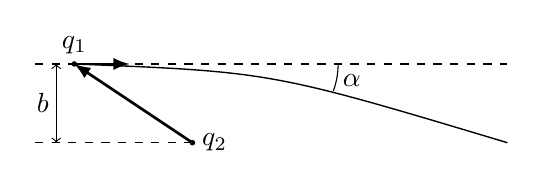
\begin{tikzpicture}


    \fill (.5,0) circle (1pt) node[above] {$q_1$};
    \fill (2,-1) circle (1pt) node[right] {$q_2$};

    \draw[dashed] (0,0) -- (6,0);
    \draw[dashed] (0,-1) -- (2,-1);

    \draw[>=latex, ->, line width=1pt] (.5,0) -- (1.2,0);

    \draw[<->] (.27,0) -- (.27, -1);
    \path (.1,-.5) node{$b$};

    % \draw (1,0) .. controls +(0:.2cm) and +(150:.8cm) .. (6,-.5);
    \draw[line width=.5pt] (.5,0) .. controls (3,-.1) .. (6,-1);

    \draw[>=latex, ->, line width=1pt] (2,-1) -- (.5,0);


    \draw (2.85,0) +(0:1cm) arc (0:-20:1cm);
    \path (3.3,-.4) ++(15:.75cm) node{$\alpha$};

\end{tikzpicture}
% end

\end{document}
